\chapter{Experimental Setup and Methods}
\label{ch:methods}

The test program was organized around three demands on a detachable supply:
hold the selected voltage under load, reduce transfer when the load disappears,
and manage the resulting electrical and thermal stress. The setup monitored both
secondary-bulk and USB-C output voltage. External instruments supplied
the output-power measurements; controller telemetry was used for diagnostics. This chapter describes the setup and
use of the instruments. Chapter~\ref{ch:results} reports the measured behavior
and the tests still needed for a continuous rating.

\section{Test Objectives and Configuration}
\label{sec:method-objectives}

The test campaign assessed loaded regulation, startup, load removal, and
no-load energy control. Input power quality, efficiency, switching waveforms,
and surface temperatures were measured to identify operating limits and
priorities for the next revision.

The V1.0 PCB was tested with two series resonant inductors. V1.1 is the corrected
schematic reference. The baseline voltage-control firmware is described in Section~\ref{sec:ctrl-firmware-identities}. Where available,
UART \texttt{VER}, \texttt{STATUS}, and \texttt{EXPORT} output identify the
active version, mode, calibration, and thresholds for comparisons of burst
operation.

\begin{table}[htbp]
\centering
\caption{Prototype tests and measurement objectives.}
\label{tab:method-objectives}
\begin{tabularx}{\textwidth}{@{}p{0.31\textwidth}X@{}}
\toprule
Question & Measured quantities\\
\midrule
Output capability & VBUS, load current, and delivered output power\\
Control response & Output voltage and PA10 during startup, steady operation, and load removal\\
Input-current shaping & Input voltage/current, real power, PF, THD, and harmonics\\
Conversion loss & Input and output power at the same recorded operating condition\\
Switching condition & Switch-node, command, and current waveforms where available\\
Thermal behavior & Surface-temperature markers and their locations at recorded loads\\
\bottomrule
\end{tabularx}
\end{table}

The measurements were obtained during supervised prototype tests. USB-PD interoperability,
standardized safety and electromagnetic-emissions qualification, and a full
soft-switching map over input and load require separate test programs.

\section{Power-Up and Test Precautions}
\label{sec:method-safety}

Bring-up used a controlled, current-limited source, rated probes, separation
from exposed conductors, and an external input disconnect. Hardware, source,
load, and probe references were checked with the burst-enable output PA10
inhibited; UART and oscilloscope connections were completed before energizing.
Probe differential and common-mode ratings were observed, and grounded
passive-probe clips were excluded from line-referenced nodes. Source isolation
did not remove shared-reference constraints.

Shutdown removed input power and the enable command. Residual DC-link and
output-capacitor voltages were checked before handling. PA10 inhibition stops
commanded transfer but does not discharge stored energy. The external
disconnect provided an emergency stop independent of UART communication.

\begin{table}[htbp]
\centering
\caption{Connections and settings needed for powered tests.}
\label{tab:method-safety-metadata}
\begin{tabularx}{\textwidth}{@{}p{0.25\textwidth}X@{}}
\toprule
Item & Settings and connections\\
\midrule
Input source & Voltage, frequency, current limit, and isolation/reference arrangement\\
Probe connection & Node pair, attenuation/range, and voltage/common-mode rating\\
Output load & Load mode, setpoint, selected output setting, and connection state\\
Shutdown & External disconnect and PA10 inhibit state\\
Stored energy & Discharge interval and verified residual voltage at accessible nodes\\
\bottomrule
\end{tabularx}
\end{table}

\section{Bench and Instruments}
\label{sec:method-bench}

The converter was supplied by the ITECH IT-M7723 programmable source. The
selected fixed output was connected to an ITECH IT8512+ electronic load or the
USB-C sink arrangement. A PC UART terminal was used to command the controller
and collect diagnostics. Load demand was set independently of the controller's
load estimate.

\begin{figure}[htbp]
\centering
\begin{subfigure}[t]{0.48\textwidth}
\centering
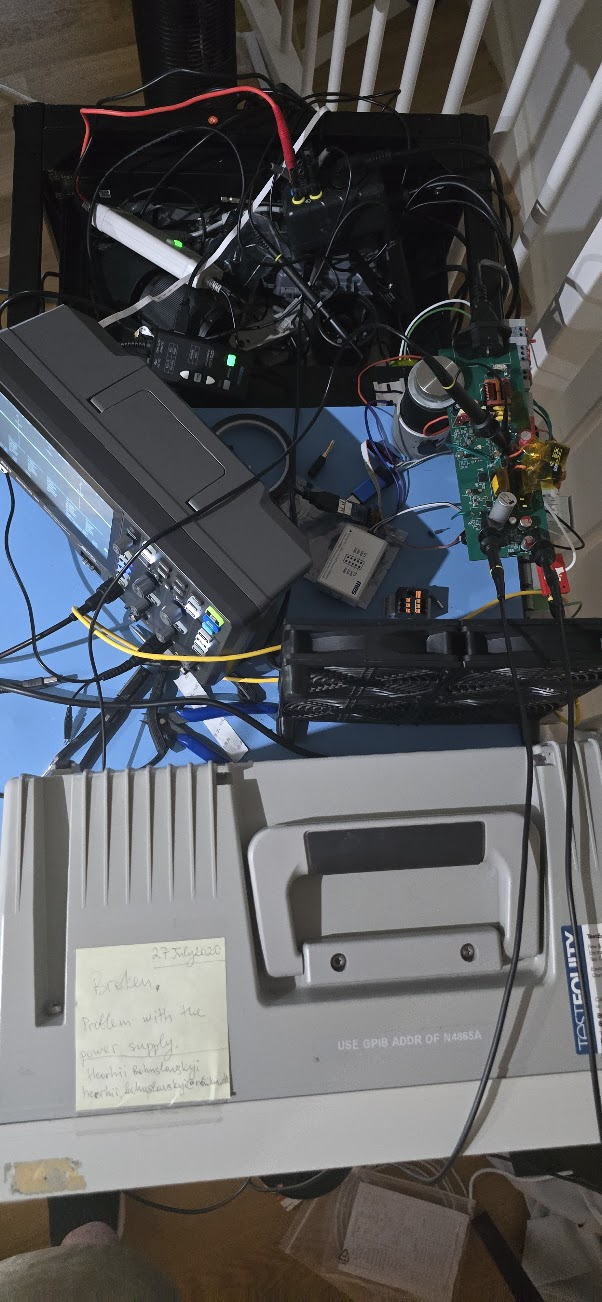
\includegraphics[width=\textwidth]{Pictures/Thesis/09_Methods/test_bench_overview_photo.png}
\caption{Source, load, and measurement arrangement.}
\label{fig:test-bench-overview-photo}
\end{subfigure}
\hfill
\begin{subfigure}[t]{0.48\textwidth}
\centering
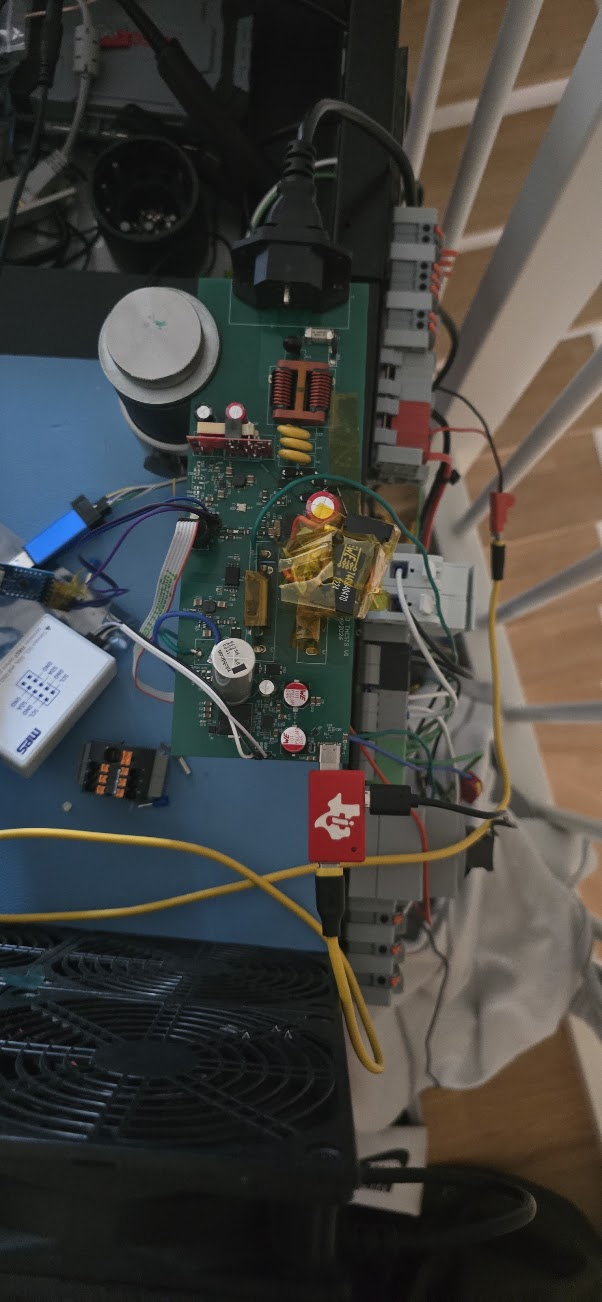
\includegraphics[width=\textwidth]{Pictures/Thesis/09_Methods/dut_probe_closeup_photo.png}
\caption{Probe access at the converter.}
\label{fig:dut-probe-closeup-photo}
\end{subfigure}
\caption{Test bench and probe connections.}
\label{fig:method-bench-photos}
\end{figure}

For input power and harmonics, the Siglent SDS824X HD was used with a Micsig
DP10013 differential voltage probe and CP2100A current probe. Switching and
output-voltage events were captured with the Keysight MSO9254A. The project
notes list February 2, 2026 as the calibration date for the main source, load,
oscilloscopes, and listed probes. Instrument serial numbers and calibration certificates
were not available.

\begin{table}[htbp]
\centering
\caption{Test equipment.}
\label{tab:bench-equipment}
\small
\begin{tabularx}{\textwidth}{@{}p{0.23\textwidth}p{0.34\textwidth}X@{}}
\toprule
Equipment & Model or range & Role\\
\midrule
Programmable source & ITECH IT-M7723 & Controlled AC input\\
Electronic load & ITECH IT8512+; \SI{120}{\volt}, \SI{30}{\ampere}, \SI{300}{\watt} & Steady and dynamic loading\\
Power-analysis oscilloscope & Siglent SDS824X HD & RMS, real power, PF, THD, and harmonics\\
Time-domain oscilloscope & Keysight MSO9254A & Switching and output events\\
Differential voltage probe & Micsig DP10013; \SI{100}{\mega\hertz}, 50X/500X & Input and high-voltage differential measurements\\
Current probe & Micsig CP2100A; DC--\SI{800}{\kilo\hertz} & Input or selected branch current\\
UART connection & \SI{115200}{baud} & Configuration, operating state, and firmware timing\\
\bottomrule
\end{tabularx}
\end{table}

Where practical, input power was measured at the DUT terminals, including
internally supplied auxiliaries. Output results identify the secondary-bulk,
connector-VBUS, or load-sense location; measurements beyond the cable include
its voltage drop and loss.

\subsection{Channel Definitions and Scaling}
\label{sec:method-instruments}

External instruments measured delivered voltage, current, and power.
ADC readings and UART data were used to diagnose controller sensing and
command handling.

\begin{table}[htbp]
\centering
\caption{Instruments and recorded measurements.}
\label{tab:instrument-role-map}
\begin{tabularx}{\textwidth}{@{}p{0.29\textwidth}p{0.30\textwidth}X@{}}
\toprule
Quantity & Instrument & Recorded output\\
\midrule
Input voltage/current and power quality & SDS824X HD with DP10013/CP2100A & Waveforms and power-analysis readings\\
Switching and load events & MSO9254A & Time-domain captures\\
Output loading & IT8512+ or USB-C sink & Load setting and voltage/current readings\\
Controller state & UART terminal & Version, settings, timing, and fault status\\
Temperature & Thermal camera & Screenshot markers and hotspot location\\
\bottomrule
\end{tabularx}
\end{table}

In Table~\ref{tab:channel-definitions}, CH1--CH4 label the oscilloscope inputs.

\begin{table}[htbp]
\centering
\caption{Typical oscilloscope channel assignments.}
\label{tab:channel-definitions}
\begin{tabularx}{\textwidth}{@{}p{0.13\textwidth}p{0.31\textwidth}X@{}}
\toprule
Channel & Quantity & Connection/scaling\\
\midrule
CH1 & Switch-node voltage & 100:1 high-voltage channel referenced to the measured circuit\\
CH2 & Secondary-bulk voltage & 10:1 voltage probe at the bulk node\\
CH3 & Connector VBUS & 10:1 probe at the output node\\
CH4 & PA10, current, or event marker & Assigned according to the event\\
\bottomrule
\end{tabularx}
\end{table}

\begin{table}[htbp]
\centering
\caption{Oscilloscope channels for input-power measurements.}
\label{tab:power-analysis-channel-definitions}
\begin{tabularx}{\textwidth}{@{}p{0.13\textwidth}p{0.30\textwidth}X@{}}
\toprule
Channel & Quantity & Connection\\
\midrule
CH1 & Input voltage & DP10013 across the DUT input\\
CH2 & Input current & CP2100A around the input conductor\\
Power application & Derived quantities & Channel scaling, polarity, averaging, and harmonic settings\\
\bottomrule
\end{tabularx}
\end{table}

Waveform interpretation requires the node assignments, probe attenuation,
range, coupling, bandwidth, trigger, and timebase for each capture. Channel
color and number alone do not identify the measurement.

\section{High-Frequency Probing}
\label{sec:method-probing}

Short local-return connections limited probe pickup and loop inductance.
Gate-source measurements require a source-referenced probe; switch-node
measurements require the full primary common-mode rating. Current-probe zero
and polarity were checked before acquisition. Voltage/current deskew is
required for switching-energy calculations. The CP2100A bandwidth of
\SI{800}{\kilo\hertz} is below the nominal \SI{1}{\mega\hertz} carrier,
limiting its use to input-current behavior rather than fast resonant-current
transitions.

A turn-on check needs switch-node voltage, the relevant gate or driver command,
and current direction through dead time to show whether the node reached the
required rail. The residual voltage at the intended turn-on instant is
\begin{equation}
 V_{\mathrm{res}}=
 \left|V_{\mathrm{SW}}(t_{\mathrm{on}})
 -V_{\mathrm{rail,target}}\right|.
 \label{eq:zvs-residual-method}
\end{equation}
The original prototype's burst-enable output PA10 marks the switching envelope,
not individual gate transitions. Enable and switch-node traces alone therefore
do not locate the ZVS measurement instant.

\begin{table}[htbp]
\centering
\caption{Probe and trigger settings needed for each test.}
\label{tab:probe-role-map}
\begin{tabularx}{\textwidth}{@{}p{0.27\textwidth}X@{}}
\toprule
Test & Probe and acquisition settings\\
\midrule
Startup/shutdown & Initial voltage, load, PA10 state, and trigger\\
Ripple/transient & Output node, probe coupling/bandwidth, sense point, and load event\\
No load/load removal & Disconnect method, output node, enable signal, and time span\\
Switching/ZVS & Gate/source reference, current direction, deskew, and bandwidth\\
Input power quality & Probe ranges, current zero/polarity, integration interval, and harmonic range\\
\bottomrule
\end{tabularx}
\end{table}

\section{Test Program and Data}
\label{sec:method-matrix}

Switching and power transfer were checked during bring-up, followed by loaded and
no-load characterization.

\begin{table}[htbp]
\centering
\caption{Prototype test program.}
\label{tab:master-test-matrix}
\begin{tabularx}{\textwidth}{@{}p{0.25\textwidth}p{0.31\textwidth}X@{}}
\toprule
Test & Controlled condition & Main observations\\
\midrule
Bring-up & Limited input and selected load & Carrier, PA10, auxiliary rails, and basic transfer\\
Startup/shutdown & Initial voltage, load, and mode & Output rise/decay and enable transitions\\
Steady output & Fixed output setting and load & Voltage, ripple, current, and power\\
Load event & Attachment or removal of load & Voltage excursion and subsequent control response\\
No load & Open output at a selected setting & Bulk/output voltage and burst pattern\\
Power quality & Recorded AC input and output condition & Real power, PF, THD, and harmonics\\
Efficiency & Matched operating-point readings & AC input and DC output power\\
Thermal & Recorded output setting and load & Surface temperatures and location\\
Switching & Selected line and load point & Switch-node, command, and current where available\\
\bottomrule
\end{tabularx}
\end{table}

Missing setup details and peak markers limit the calculations, as discussed in
\cref{sec:method-uncertainty}. Plot lines connect measured points and are not
fitted converter characteristics.

\subsection{Control, No-Load, and Load-Removal Tests}
\label{sec:method-control}

The final baseline controller acquired secondary-bulk voltage at PA1 through
continuous ADC DMA and controlled switching intervals through the MCU burst-enable
pin PA10. Saved UART settings, where available, identified the active
configuration rather than source-code defaults.

Loaded tests checked delivered voltage and burst structure at a fixed output setting. Because the records begin after startup, synchronized measurements of initial conditions, precharge, output rise and peak, the burst-enable signal (PA10), inhibition, decay, and fault status are still needed to quantify startup and shutdown.

Load-removal captures covered output voltage and switching around disconnection.
A complete assessment requires both the immediate stored-energy response and
later no-load cycling, with thresholds, latch state, and recovery recorded to
distinguish holdoff from a latched fault.

\begin{table}[htbp]
\centering
\caption{Signals needed for control-response tests.}
\label{tab:control-tests}
\begin{tabularx}{\textwidth}{@{}p{0.27\textwidth}X@{}}
\toprule
Condition & Observations\\
\midrule
Startup & Initial state, precharge, output rise, maximum voltage, and fault status\\
Loaded operation & Output voltage/ripple, load current, and PA10 pattern\\
Load removal & Immediate voltage excursion, enable response, and final no-load behavior\\
No load & Complete/partial burst structure and voltage cycling\\
Protection event & Calibrated threshold, inhibition, latch/holdoff state, and recovery\\
\bottomrule
\end{tabularx}
\end{table}

\section{Input Power Quality}
\label{sec:method-pq}

Input-current shaping under burst control was assessed using the SDS824X HD,
DP10013, and CP2100A. The recorded quantities were RMS voltage/current, real
input power, true power factor, and input-current THD:
\begin{equation}
 \mathrm{PF}=\frac{P_{\mathrm{in}}}
 {V_{\mathrm{in,rms}}I_{\mathrm{in,rms}}},
 \label{eq:pf-method}
\end{equation}
\begin{equation}
 \mathrm{THD}_I=
 \frac{\sqrt{\sum_{h=2}^{N}I_h^2}}{I_1}.
 \label{eq:thd-method}
\end{equation}
The percentage is \(100\,\mathrm{THD}_I\), with the harmonic range set by the
analyzer's selected value of \(N\).

Steady-state integration must cover several line cycles and representative
burst activity, excluding startup and load transitions. Source isolation and
input current limiting remain part of the test configuration. PF, current
waveform, and THD were compared at the same operating condition; no
harmonics-standard qualification was performed.

\section{Conversion Efficiency}
\label{sec:method-efficiency}

System efficiency was calculated from real AC input power and DC power at the
stated output measurement point:
\begin{equation}
 \eta_{\mathrm{sys}}=
 \frac{P_{\mathrm{out}}}{P_{\mathrm{in}}}\,100\%.
 \label{eq:efficiency-method}
\end{equation}
For steady voltage and current readings, output power is
\begin{equation}
 P_{\mathrm{out}}=V_{\mathrm{out}}I_{\mathrm{out}}.
 \label{eq:pout-method}
\end{equation}
For a changing waveform, the calculation instead needs the average of the
instantaneous product \(v(t)i(t)\).

For the V2 secondary-load tests, the AC supply's reported real power was
paired with voltage and current at the electronic-load terminals. Their
product gives the secondary-load power used in the efficiency estimate.
Loss in the leads between the secondary output and load is included with
the converter losses; no cable-loss correction was applied.

Paired entries use the same operating condition. DUT input measurements include
internal auxiliaries; the stated output sense point determines cable-loss
inclusion. No cable-loss correction was made without a measured voltage drop.
The results in Chapter~\ref{ch:results} are initial estimates because a
synchronized, repeated sweep with a complete uncertainty budget was not
available at every point. Unmatched observations were excluded.

\section{Thermal Imaging}
\label{sec:method-thermal}

Thermal images recorded labeled voltage/current conditions and maximum,
cursor, and reference-marker temperatures at emissivity 0.95. The images
locate apparent surface hotspots; viewing angle, reflections, focus, and
component visibility affect the readings. Junction temperature and individual
copper, winding, and core losses cannot be extracted.

For the V2 secondary-load sequence, region R3 covered the input bridge and
R1 the secondary area. The maximum surface temperature in each region was
read with the displayed region emissivity of 0.95. Thermal images and
electrical readings were paired in test order and were taken a few seconds
apart.

Ambient, airflow, warm-up, and camera setup were not fully recorded.
The identified hotspots can be monitored during longer runs.

\section{Measurement Uncertainty and Repeatability}
\label{sec:method-uncertainty}

Relevant uncertainties include instrument accuracy, probe attenuation and
zero, voltage/current phase error, channel timing, output sense location,
cable drop, emissivity, and repeatability. ADC scaling and thresholds can
also shift burst operation and the operating point.

For independent measured inputs \(x_i\), the combined standard uncertainty
of a calculated quantity \(y\) is
\begin{equation}
 u_c(y)=
 \sqrt{\sum_i
 \left(\frac{\partial y}{\partial x_i}u(x_i)\right)^2}.
 \label{eq:uncertainty-propagation}
\end{equation}
For output power and efficiency, this gives
\begin{equation}
 \frac{u(P_{\mathrm{out}})}{P_{\mathrm{out}}}
 =
 \sqrt{\left(\frac{u(V_{\mathrm{out}})}{V_{\mathrm{out}}}\right)^2+
 \left(\frac{u(I_{\mathrm{out}})}{I_{\mathrm{out}}}\right)^2},
 \label{eq:pout-uncertainty}
\end{equation}
\begin{equation}
 \frac{u(\eta)}{\eta}
 =
 \sqrt{\left(\frac{u(P_{\mathrm{out}})}{P_{\mathrm{out}}}\right)^2+
 \left(\frac{u(P_{\mathrm{in}})}{P_{\mathrm{in}}}\right)^2}.
 \label{eq:eta-uncertainty}
\end{equation}
Correlated inputs require covariance terms in addition to these simplified
independent-input expressions.

The setup information and repeated measurements needed for a numerical uncertainty budget are incomplete, so no error bars are given. Characterizing worst-case transients requires repeated events with a defined acceptance band; thermal equilibrium requires a temperature history, and jitter requires timing measurements. These limits apply throughout Chapter~\ref{ch:results}.

\section{Remaining Tests in the Revised Plan}
\label{sec:method-plan-validation}

The remaining campaign targets a repeatable V2 baseline, power-limit diagnosis,
and a matched V3 comparison \cite{projectOctoberPlan}. AP-01--AP-08 are defined
in Section~\ref{sec:revised-plan-criteria}; current results are summarized in
Section~\ref{sec:res-revised-plan}.

\subsection{Repeat the V2 Baseline}

The reported V2 operating point near \SI{85}{\watt} must be repeated with
the hardware, rework, magnetics, resonant values, controller target, firmware version, settings and mode
identified. AC input, output setting and negotiation, load and cable, auxiliary
supplies, cooling, ambient and duration must also be recorded. Probe scaling
and zero must be checked. If the original configuration cannot be reconstructed,
the known differences must be stated.

The measurements must identify the analyzer, ranges and accuracy,
probe positions, bandwidth, averaging and timing, and thermal sensing method.
Protocol tests must identify advertised capabilities and requested/accepted
sink settings.

\subsection{Power and Temperature Measurements}

Real AC input power, external connector voltage, and load current must be
measured over the same steady interval for the calculation in
Section~\ref{sec:method-efficiency}. Secondary-bulk measurements and the
primary-current input PA2 describe upstream control rather than connector
output power. The boundary must include internally supplied auxiliaries and
measured external supply power, with any exclusions stated.

Instrument ranges, scaling, calibration, and the propagation method in
Section~\ref{sec:method-uncertainty} define the uncertainty. Unmatched
averaging windows, changing load, or omitted auxiliary power invalidate a
matched efficiency estimate.

Continuous-power tests require a specified duration, thermal-stability
criterion, and numerical stop limits. Initial condition, elapsed time,
ambient, airflow, orientation, heat sinks, and temperature histories must be
recorded; isolated electrical and thermal captures are insufficient.

\subsection{Staged Loading and Controlled Changes}

The planned sequence in Table~\ref{tab:method-revised-load-sequence} is limited
by the selected PDO/APDO and cable, connector, load, and converter ratings.
Unsupported voltage/current combinations must be omitted or reconfigured.

\begin{table}[H]
\centering
\small
\caption[Planned load sequence.]{Planned load sequence for the remaining tests.}
\label{tab:method-revised-load-sequence}
\begin{tabularx}{\textwidth}{@{}L{0.28\textwidth}Y@{}}
\toprule
Stage & Test and condition for increasing load\\
\midrule
\SI{25}{\watt}, \SI{45}{\watt}, \SI{65}{\watt} & Measure regulation, power quality, efficiency, stress, and heating at increasing load under an applicable output setting.\\
\SI{75}{\watt}, \SI{80}{\watt}, approximately \SI{85}{\watt} & Repeat the upper baseline range and document whether the plan's V2 point is reproduced.\\
\SI{90}{\watt}, \SI{95}{\watt}, \SI{100}{\watt} & Proceed in stages only after the previous point passes the defined stress, temperature, control, and interface checks.\\
Final stable point & Complete the defined-duration thermal/stability run and the full measurement set; report the highest repeatable power if the target is not reached.\\
\bottomrule
\end{tabularx}
\end{table}

Stop limits must follow component ratings, expected stress, sensing range,
and thermal assumptions, with surface and junction limits treated separately.
Limit crossings, loss of regulation/feedback, unexplained protection, or
abnormal switching require termination and a saved event trace.

Controlled retests must change one item while retaining the remaining setup.
The log must identify the part or setting, rationale, expected effect, and
before/after records. Candidates include sensing calibration, control limits,
switching timing, resonant and charge-pump values, gate behavior, conduction
paths, rectification, and cooling. Calibration changes require raw readings
and both scales to separate display correction from electrical improvement.

\subsection{Output, Transient, and Thermal Tests}

Fixed-PDO tests must record advertised and negotiated voltage/current,
regulation, load range, and attach/detach behavior. PPS tests require an
advertised APDO, requested/accepted settings, measured connector output,
transitions, and limit behavior.

Startup, shutdown, load steps/removal, no-load recovery, and mode transitions
require synchronized connector VBUS, relevant bulk/control signals, and event
markers. Protection tests must define the applied fault, trigger, response,
and recovery within the bench limits.

At the final accepted power, efficiency, PF/THD, ripple, transients, stress,
and extended thermal stability must be assessed. Drift, protection,
interruptions, and cooldown/restart behavior belong in the run record.
A defined-duration result applies to those conditions rather than lifetime
reliability.

\subsection{Comparing V2 and V3 Power Density}
\label{sec:method-density}

For both assemblies, the rectangular envelope of the complete installed
converter would be measured:
\begin{equation}
 V_{\mathrm{assembly}}=LWH,
 \qquad
 \rho_P=\frac{P_{\mathrm{out,continuous}}}{V_{\mathrm{assembly}}}.
 \label{eq:method-assembly-density}
\end{equation}
The envelope includes both PCB sides, required daughterboards/connectors,
heat sinks, and functional hardware moved off-board. Both assemblies must
use the same axes and treatment of enclosure, cooling, and supports; bench
instrumentation is excluded.

The numerator requires externally verified continuous output under stated
duration, ambient, airflow, input, output setting, and thermal conditions.
Density must be reported with efficiency, temperature, and margin. A nominal
\SI{100}{\watt} rating and a short measured peak are not comparable under AP-07.

The approximately \SI{8}{\percent} V3 reduction is a design-volume estimate
with USB-PD omitted, not a complete-supply comparison. External regulation,
PD control, connectors, and required cooling must enter the system volume.
Verified dimensions and matched continuous-power tests remain unavailable,
so no V2/V3 density result is reported. AP-08 specifies completed V2 testing
as the fallback if V3 is not ready.

